\documentclass[a4paper, 11pt]{article}
\usepackage{comment} % enables the use of multi-line comments (\ifx \fi) 
\usepackage{lipsum} %This package just generates Lorem Ipsum filler text. 
\usepackage{fullpage} % changes the margin
%\usepackage[]{algorithm2e}
\usepackage{algorithm}% http://ctan.org/pkg/algorithms
\usepackage{algpseudocode}% http://ctan.org/pkg/algorithmicx
\usepackage[para,online,flushleft]{threeparttable}
\usepackage{booktabs}
%\usepackage{cleveref}
\usepackage[utf8x]{inputenc}
\usepackage{graphicx}
\usepackage{cite}
%\renewcommand\thesubsection{\Alph{subsection}}

\def\BibTeX{{\rm B\kern-.05em{\sc i\kern-.025em b}\kern-.08em
    T\kern-.1667em\lower.7ex\hbox{E}\kern-.125emX}}

\begin{document}
%Header-Make sure you update this information!!!!
\noindent
\large\textbf{Nonholonomic Planning Assignment 3 Report} \hfill \textbf{Sean Ye, Patrick Grady} \\
\normalsize CS 8803 - Adaptive Control and Reinforcement Learning \\
Prof. Byron Boots \hfill Date: 04/15/2019 \\

\section{Overview}

For this assignment, we chose to use an RRT planner to generate feasible paths for the car to follow. The planner is able to produce paths for all maps given bridges are open but does not converge in a reasonable time to produce plans through the many tight turns on maps 2 and 3.

\section{Nonholonomic RRT Planner}

The basic RRT algorithm implemented is shown below (\ref{alg:RRT}). This algorithm was first described by LaValle in 1998 \cite{Lavalle98}. In our implementation, the map provided to the algorithm has a threshold to assume bridges were open or close. For example, if a bridge has a probability of being open greater than 70\% of the time, the planner assumes it to be open.

\begin{algorithm}[H]
    \begin{algorithmic}
    \State Initialize Tree $T$
    \While{$x_{goal}$ not reached }
    		\State $x_{rand} \leftarrow RANDOM\_STATE()$
    		\State $x_{near} \leftarrow NEAREST\_NEIGHBOR(x_{rand}, T)$
    		\State $u_{new} \leftarrow SELECT\_CONTROL(x_{rand}, x_{near})$
    		\State $x_{new} \leftarrow STEER(u_{new}, x_{near})$
    		\State $T.add\_vertex(x_{new})$
    		\State $T.add\_edge(x_{near}, x_{new}, u_{new})$
	\EndWhile    	
    \end{algorithmic}
\caption{RRT Algorithm}
\label{alg:RRT}
\end{algorithm}

Several modifications were made to this algorithm to perform better for this project. Each modification with respect to the function is listed here:

\subsection{RANDOM\_STATE()}
Rather than a completely random point chosen for the RRT, we decided to choose the goal point 15 percent of the time. This heuristically biases the tree to keep on trying to explore regions to get to the goal.

\subsection{NEAREST\_NEIGHBOR()}
The nearest neighbor function was modified so that each node in the tree kept track of how many children it has. Instead of always expanding the closest node, the algorithm instead skips nodes with more than $n$ children and chooses the next closest neighbor. This biases the exploration to try new areas of the map and avoid areas which are most likely blocked by obstacles. 

\subsection{SELECT\_CONTROL()}
Select control tests each control value from -1 to 1 in 0.1 intervals to test which point is closest to $x_{rand}$. The distance heuristic used was the Manhattan distance rather than the Eulerian distance to better represent the non-holonomic constraints of the car \cite{Li2014}. The function uses the motion model to know if the car has hit any obstacles. If the goal is reached, it immediately returns that action value. The entire RRT algorithm uses timesteps between 7 and 20. This is because a single timestep does not allow for adequate exploration of the tree. Additionally, some random noise between -0.1 and 0.1 was added to the action value.

\subsection{STEER()}
Steer uses the motion model to create the new $x_{new}$ node to add to the tree. If the motion model found a goal the algorithm immediately stops. 


\section{Results}

The performance results are summarized in Table \ref{tab:results}. The algorithm always finds the goal in Map 1 because it avoids the potential wall. On maps 2 and 3, the algorithm only fails when the potential walls are there as the planner does not take these into account. Therefore the average rounds completed is dependent on which path the RRT happens to find first and the bridge probabilities. Figure \ref{fig:maps} shows the planning process of the RRT. 

\begin{table*}[h!]
  \label{tab:results}
\begin{center}
  \begin{threeparttable}
    \caption{Results Summary}
    
     \begin{tabular*}{\textwidth}{l @{\extracolsep{\fill}} rrrr}
        \toprule
        Map \# & Average Rounds Completed & Best Performance & Worst Performance & Collision\\
        \midrule
		Map 1     & 10/10 		  & Complete Goal & N/A        &	N/A\\
		Map 2	  & 17/20 or 7/20       & Complete Goal & Hit Wall   &	Yes\\
		Map 3	  & 26/40      		  & Complete Goal & Hit Wall   &  	Yes\\
        \bottomrule
     \end{tabular*}
  \end{threeparttable}
  \end{center}
\end{table*}

\begin{figure}[h]
	\centering
	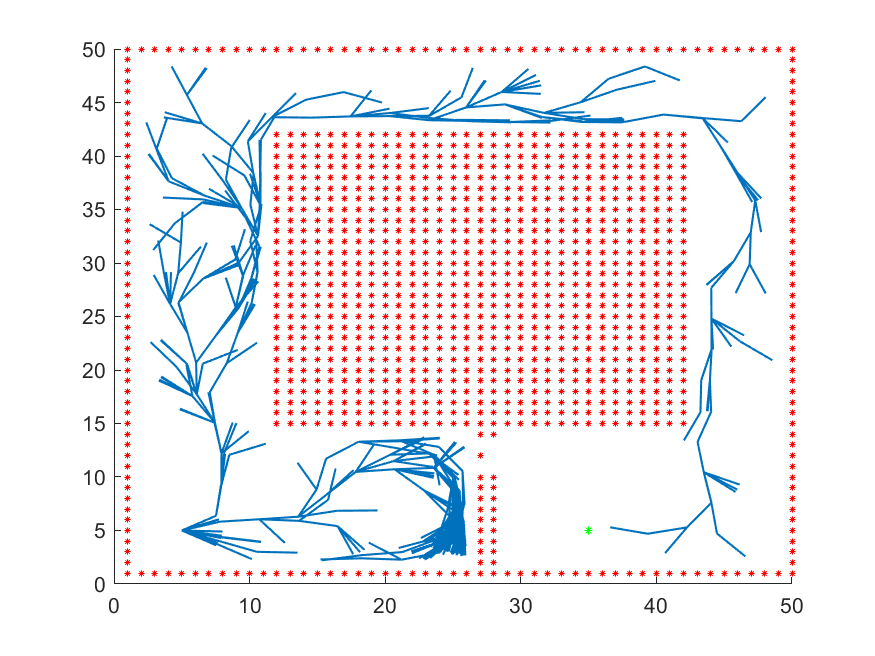
\includegraphics[scale=0.52]{../Figures/map1a.png}
	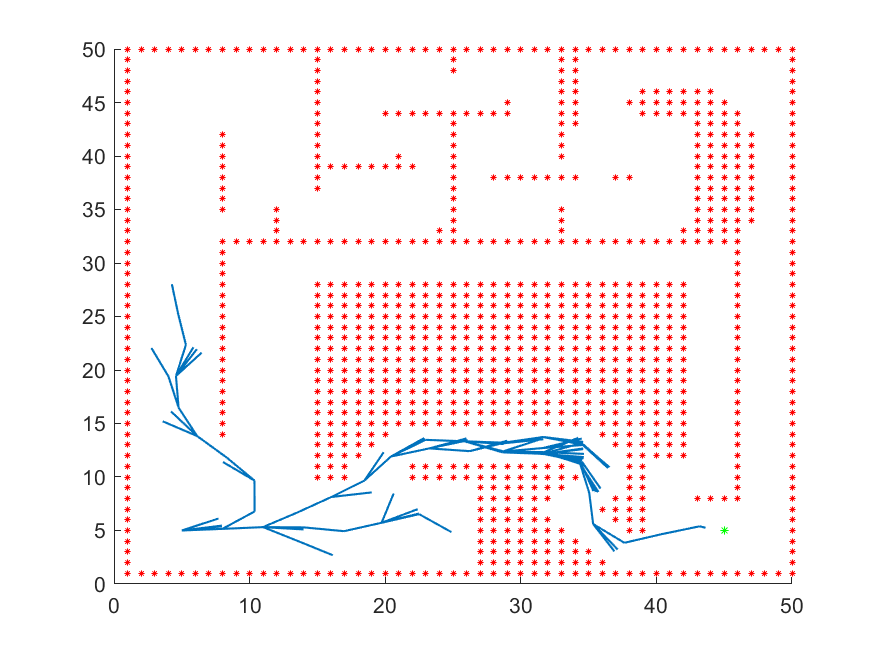
\includegraphics[scale=0.52]{../Figures/map2.png}
	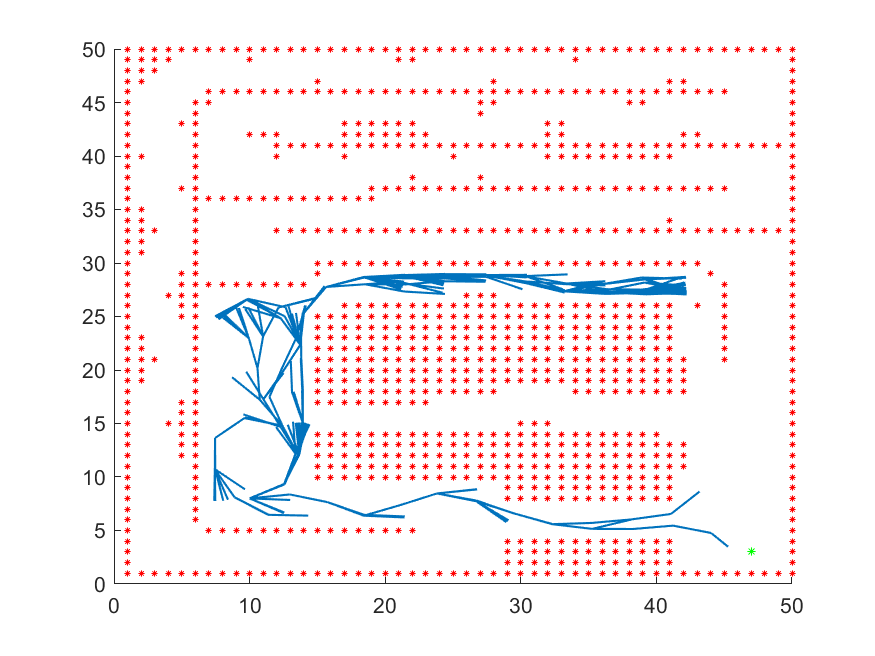
\includegraphics[scale=0.52]{../Figures/map3.png}
	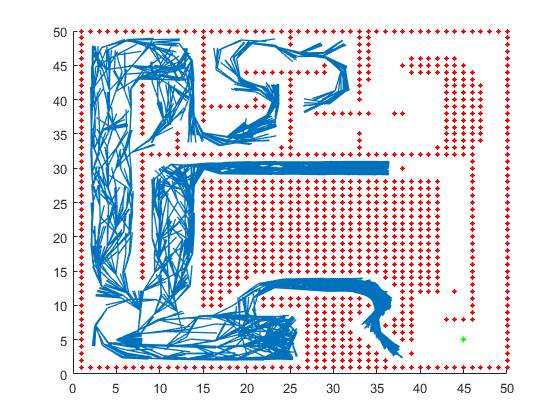
\includegraphics[scale=0.52]{../Figures/map2_fail.png}
	\caption{Plans by RRT (top left: map 1, top right: map 2, bottom left: map 3, bottom right: failed map 2)}
	\label{fig:maps}
\end{figure} 

The planner gets stuck if all the openings are blocked and the only viable path has a lot of tight curves (as seen in Figure \ref{fig:maps}). While the code has a max expansion for nodes, the problem is that the planner creates many nodes very close to each other which causes several nodes to be placed near the walls. 

%\begin{figure}[h!]
%	\centering
%	
%	\caption{Map 2 Failed RRT}
%	\label{fig:map2}
%\end{figure} 
%
%\begin{figure}[h!]
%	\centering
%	
%	\caption{Map 3 RRT}
%	\label{fig:map3}
%\end{figure} 


\section{Conclusion and Possible Modifications}

In summary, the RRT planner does well when the path between the start and goal has few tight turns or corners. There are many possible improvements to be made on the implementation here. First, you could perhaps run value iteration or A* to heuristically bias the search to the route you know is optimal \cite{Urmson2004}. RRT* could also be implemented to create more optimal paths than the ones produced here. You could also bias the random nodes placed towards open areas of the map to avoid continuously exploring regions which are blocked or are filled with nodes already. Finally, if the car detects a new obstacle, it could try and replan again by creating a new tree. However, this would involve including the backwards command into the algorithm which would require modifying how nodes are strung together if RRT* is also implemented. 


\section*{Attachments}
%Make sure to change these
Code can be run with run\_sim.m, first displays progress of RRT planner and then runs the path
%\fi %comment me out

\bibliography{RRT_bib}
\bibliographystyle{plain}

\end{document}
